\subsection{Ablation Study}
\label{sec:exp-ablation}

In this section, we explore the contributions of the various components of our system.
%All ablation results in this section are evaluated on the on the validation set.


\noindent
\textbf{Feature Variations}

We first evaluate table linking results using different feature combinations.
\tabref{tab:ablation-features} shows the results of feature ablation studies.
All features in our model make a positive effect on the final accuracy.
Both the cell feature and the context feature directly represents
the latent semantic association between the embedding of an individual mention
(either from itself or from its neighborhoods) and the candidate entity.
Among them, the cell feature is more important in the model since it encodes
the most direct information between the mention and the target entity.
We observe that when using coherence feature only, a significant decrease is incurred,
largely due to the lack of dominant and direct semantic features.
%We observe that Micro Accuracy drops when adopting these two features only,
%but it still outperforms other ablations,
Nevertheless, the coherence feature is complementary to the other features,
as it aims to discover the latent correlation in a global perspective,
modeling whether different candidate entities in one column 
are close to each other, for example, sharing the same (or similar) type,
even though no explicit type or category information is attached to the entity.
% it also shows that our coherence feature is able to extract the latent correlation
%between the target concepts, even though no explicit type or category information
%is attached to each candidate entity.

As the example shown in \figref{fig:example}, the mention 
``钢铁侠'' could be either
``Iron\_Man'' (the fictional superhero) or ``Iron\_Man\_(2008\_film)'' 
in Wikipedia, while both ``驯龙高手'' (``How\_to\_Train\_Your\_Dragon\_(film)'') and
``线人'' (``The\_Stool\_Pigeon\_(2010\_film)'') have less ambiguity.
Our model predicts the superhero when using cell + context features only.
After applying the coherence feature, 
the strong correlation between the entities in the same column
makes the model bias toward the correct film entity.


\begin{table}[ht]
    \centering
    \caption{Micro Accuracies and performance decreasing percentages
             on the validation set using different feature combinations.}
    \label{tab:ablation-features}
    \begin{tabular} {c|c|c}
        Feature Combination &   Micro Acc.  & Decrease (\%) \\
        \hline
        Cell Only           &   0.662    & 4.85 \\
        Context Only        &   0.654    & 6.06   \\
        Cell + Context      &   0.679    & 2.44    \\
        Coherence Only      &   0.228    & 67.28     \\
        \hline
        Full                &   0.696    & 0.00  \\
    \end{tabular}
\end{table}



\begin{figure}[th]
\centering
%\epsfig{file=fb-schema-4.eps, width=0.95\columnwidth}
\scalebox{0.25}{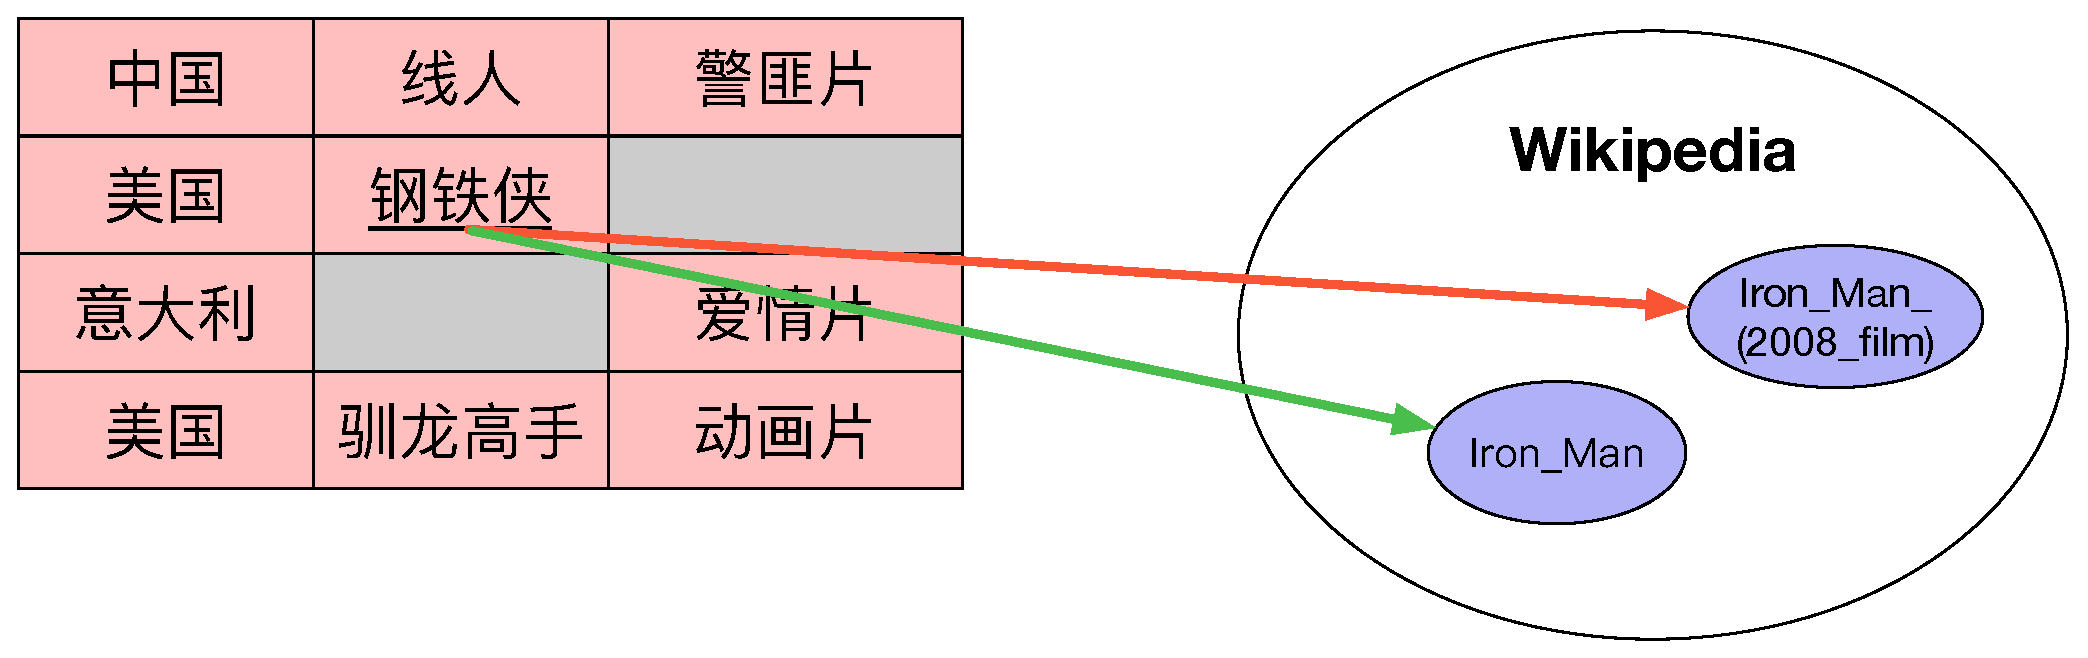
\includegraphics[angle=0]{example.eps}}
\caption{A real example of table linking. The green arrow points to the entity 
predicted without using coherence feature, and the red arrow points to the entity
predicted by using all features.}
\label{fig:example}
\end{figure}


\noindent
\textbf{Joint Model Versus Non-Joint Model}

We investigate the effect of joint model without introducing the coherence feature.
As discussed before, the cell and context features focus on relationships of individual mentions,
then we simply transform the table linking problem into a traditional entity linking problem:
given a mention's cell and context embedding (rather than a table of multiple mentions),
link the mention to an entity in the knowledge base.
Also, the gold linking result of a training table becomes a list of $(mention, entity)$ pairs.

We construct a non-joint model as the baseline: during training step, we adopt hinge loss
as the optimizing function, in order to maximize the margin $\lambda$ between the gold entity $e^+$
and other entities $e^-$ of a mention $m$, defined as follows:
\begin{equation}
\label{eqn:hinge-loss}
l_m = \max_{e^- \in Cand(m)} \max \{ 0, \lambda + score(m, e^-) - score(m, e^+) \}.
%l_{m} = \max_{e^-}ffff
\end{equation}

\noindent
In this model,  $score(\cdot, \cdot)$ is similar with \eqnref{eqn:score},
but remove the coherence feature, and don't need to average cell and context features over mentions.
The parameter $\lambda$ is tuned in \{1.0, 2.0, 3.0, 4.0\}.
We also perform another ablation test, where we apply the joint model,
but the pairwise rank loss is replaced by the hinge loss.

\tabref{tab:ablation-joint} shows the comparison of Micro Accuracy on the testing set.
We find out that when both using hinge loss, the non-joint model outperforms
the joint model.
We believe that hinge loss is not suitable for use in our joint model,
because: 1) all the negative candidates of each mention are used in the non-joint model,
however, in the joint model, negative entity tables are generated by random corruption (see \secref{sec:strategy}),
some negative candidates are not sampled and hence cannot be observed by the model;
2) hinge loss focus on the margin between the positive entity table and the nearest negative entity
table (only a few corruption), thus many negative tables with many corruptions become unimportant,
which shrinks the size of training data to some extent.
Compared with the hinge loss, the pairwise ranking model imposes the intuition
that the more corruption a table has, the lower score it holds.
Once negative entity tables are comparable of each other, the training model
could make full use of negative entity tables.

\begin{table}[ht]
    \centering
    \caption{Experimental results on the testing set under different model specification.
             Only mention features and context features are used in each model.}
    \label{tab:ablation-joint}
    \begin{tabular} {c|c|c}
        Specification &   Micro Acc.  & Decrease (\%) \\
        \hline
        Non-Joint, Hinge Loss &   0.586        &  2.01     \\
        Joint, Hinge Loss     &   0.574        &  4.01     \\
        Joint, RankNet        &   0.598        &  0.00     \\
    \end{tabular}
\end{table}



%\textbf{Effect of pre-train data size.}
%Train on the common word dataset.
%Show experimental results, based on non-joint model.
%
%1) size of words, cosine similarity in test, final result
%
%2) or draw a figure, showing non-joint and joint accuracy trend.
%

